\subsection{Red Doméstica}

Para la primera captura, se eligió la red domestica de uno de los integrantes del grupo. Los dispositivos conectados a la red en este caso fueron, 3 computadoras, 2 teléfonos celulares, un televisor SmartTV y un Apple TV. Todos estos conectados al modem del proveedor de internet.
La captura se realizó desde la computadora con dirección IP 192.168.0.30 mediante conexión WIFI y la misma duró aproximadamente 30 minutos.

\FloatBarrier

\subsubsection{Paquetes capturados e información}

A continuación analizaremos la relación entre la cantidad de paquetes y la información que provee cada tipo de protocolo de la fuente $S$.

\begin{figure}[ht!]
  \centering
  \begin{minipage}[b]{0.48\textwidth}
    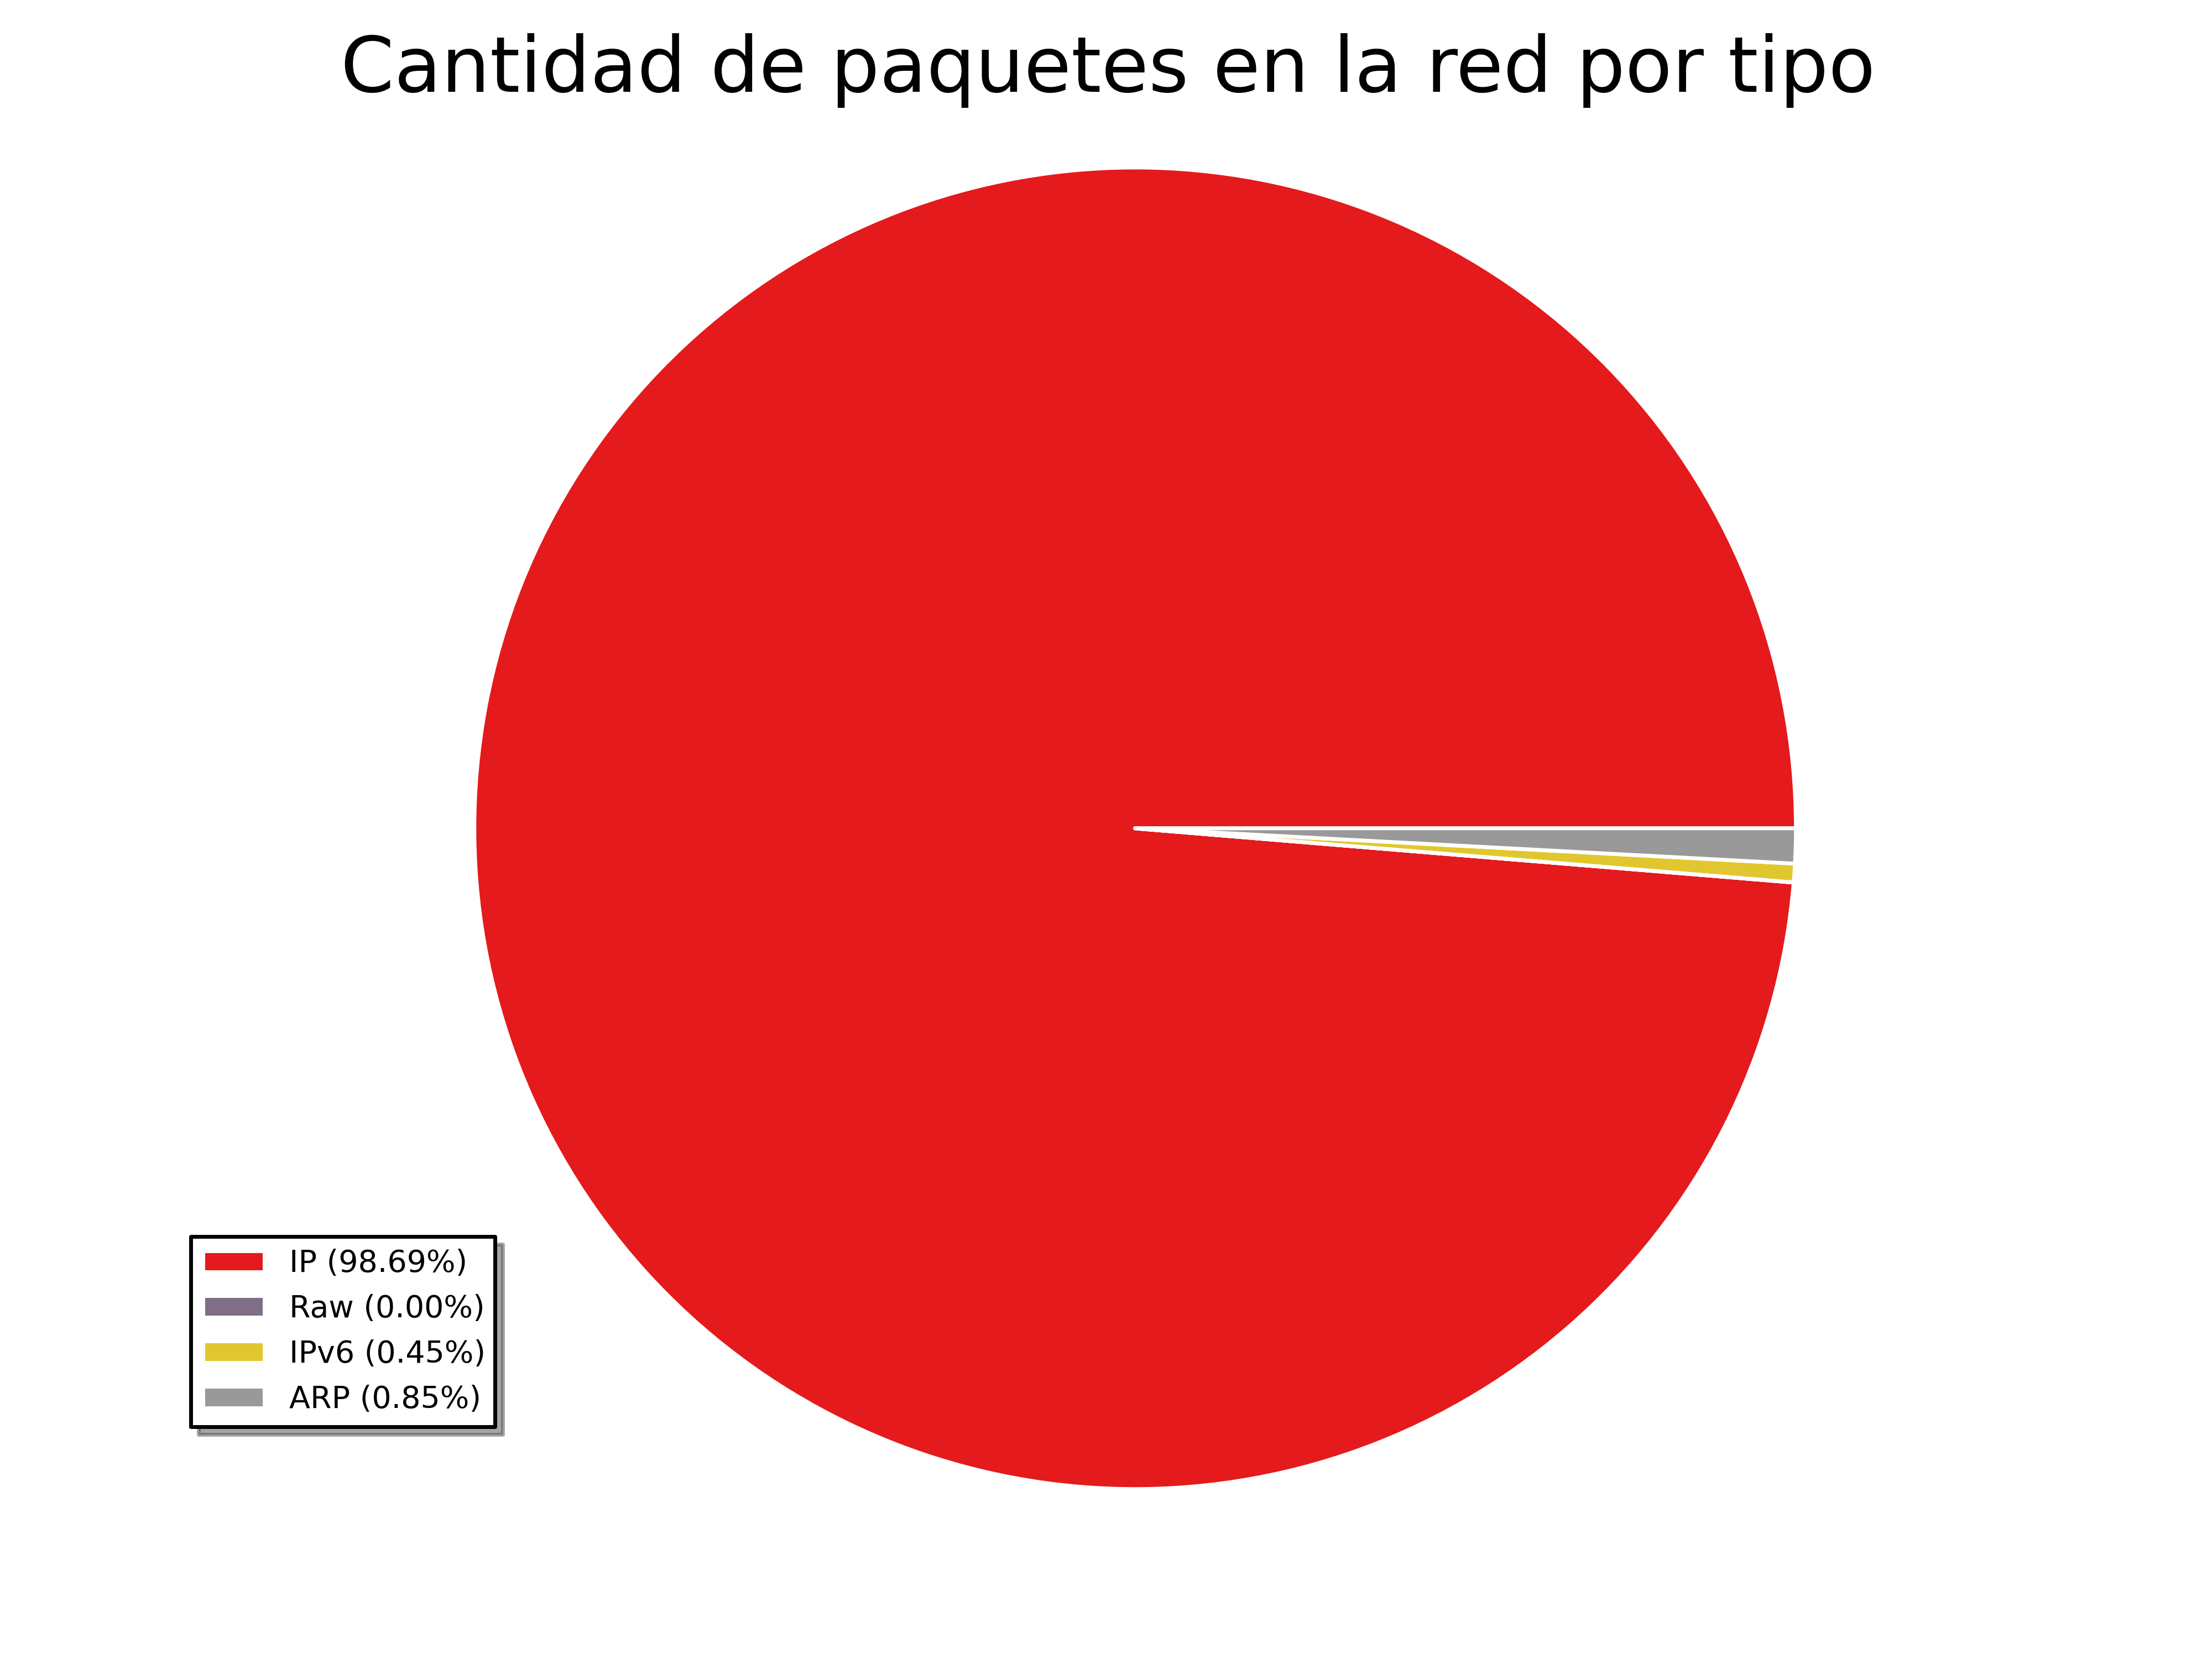
\includegraphics[width=\textwidth]{graficos/red_domestica_pie_type.png}
    \caption{Fuente $S$}
    \label{fig:red_domestica_pie_type}
  \end{minipage}
  \hfill
  \begin{minipage}[b]{0.48\textwidth}
    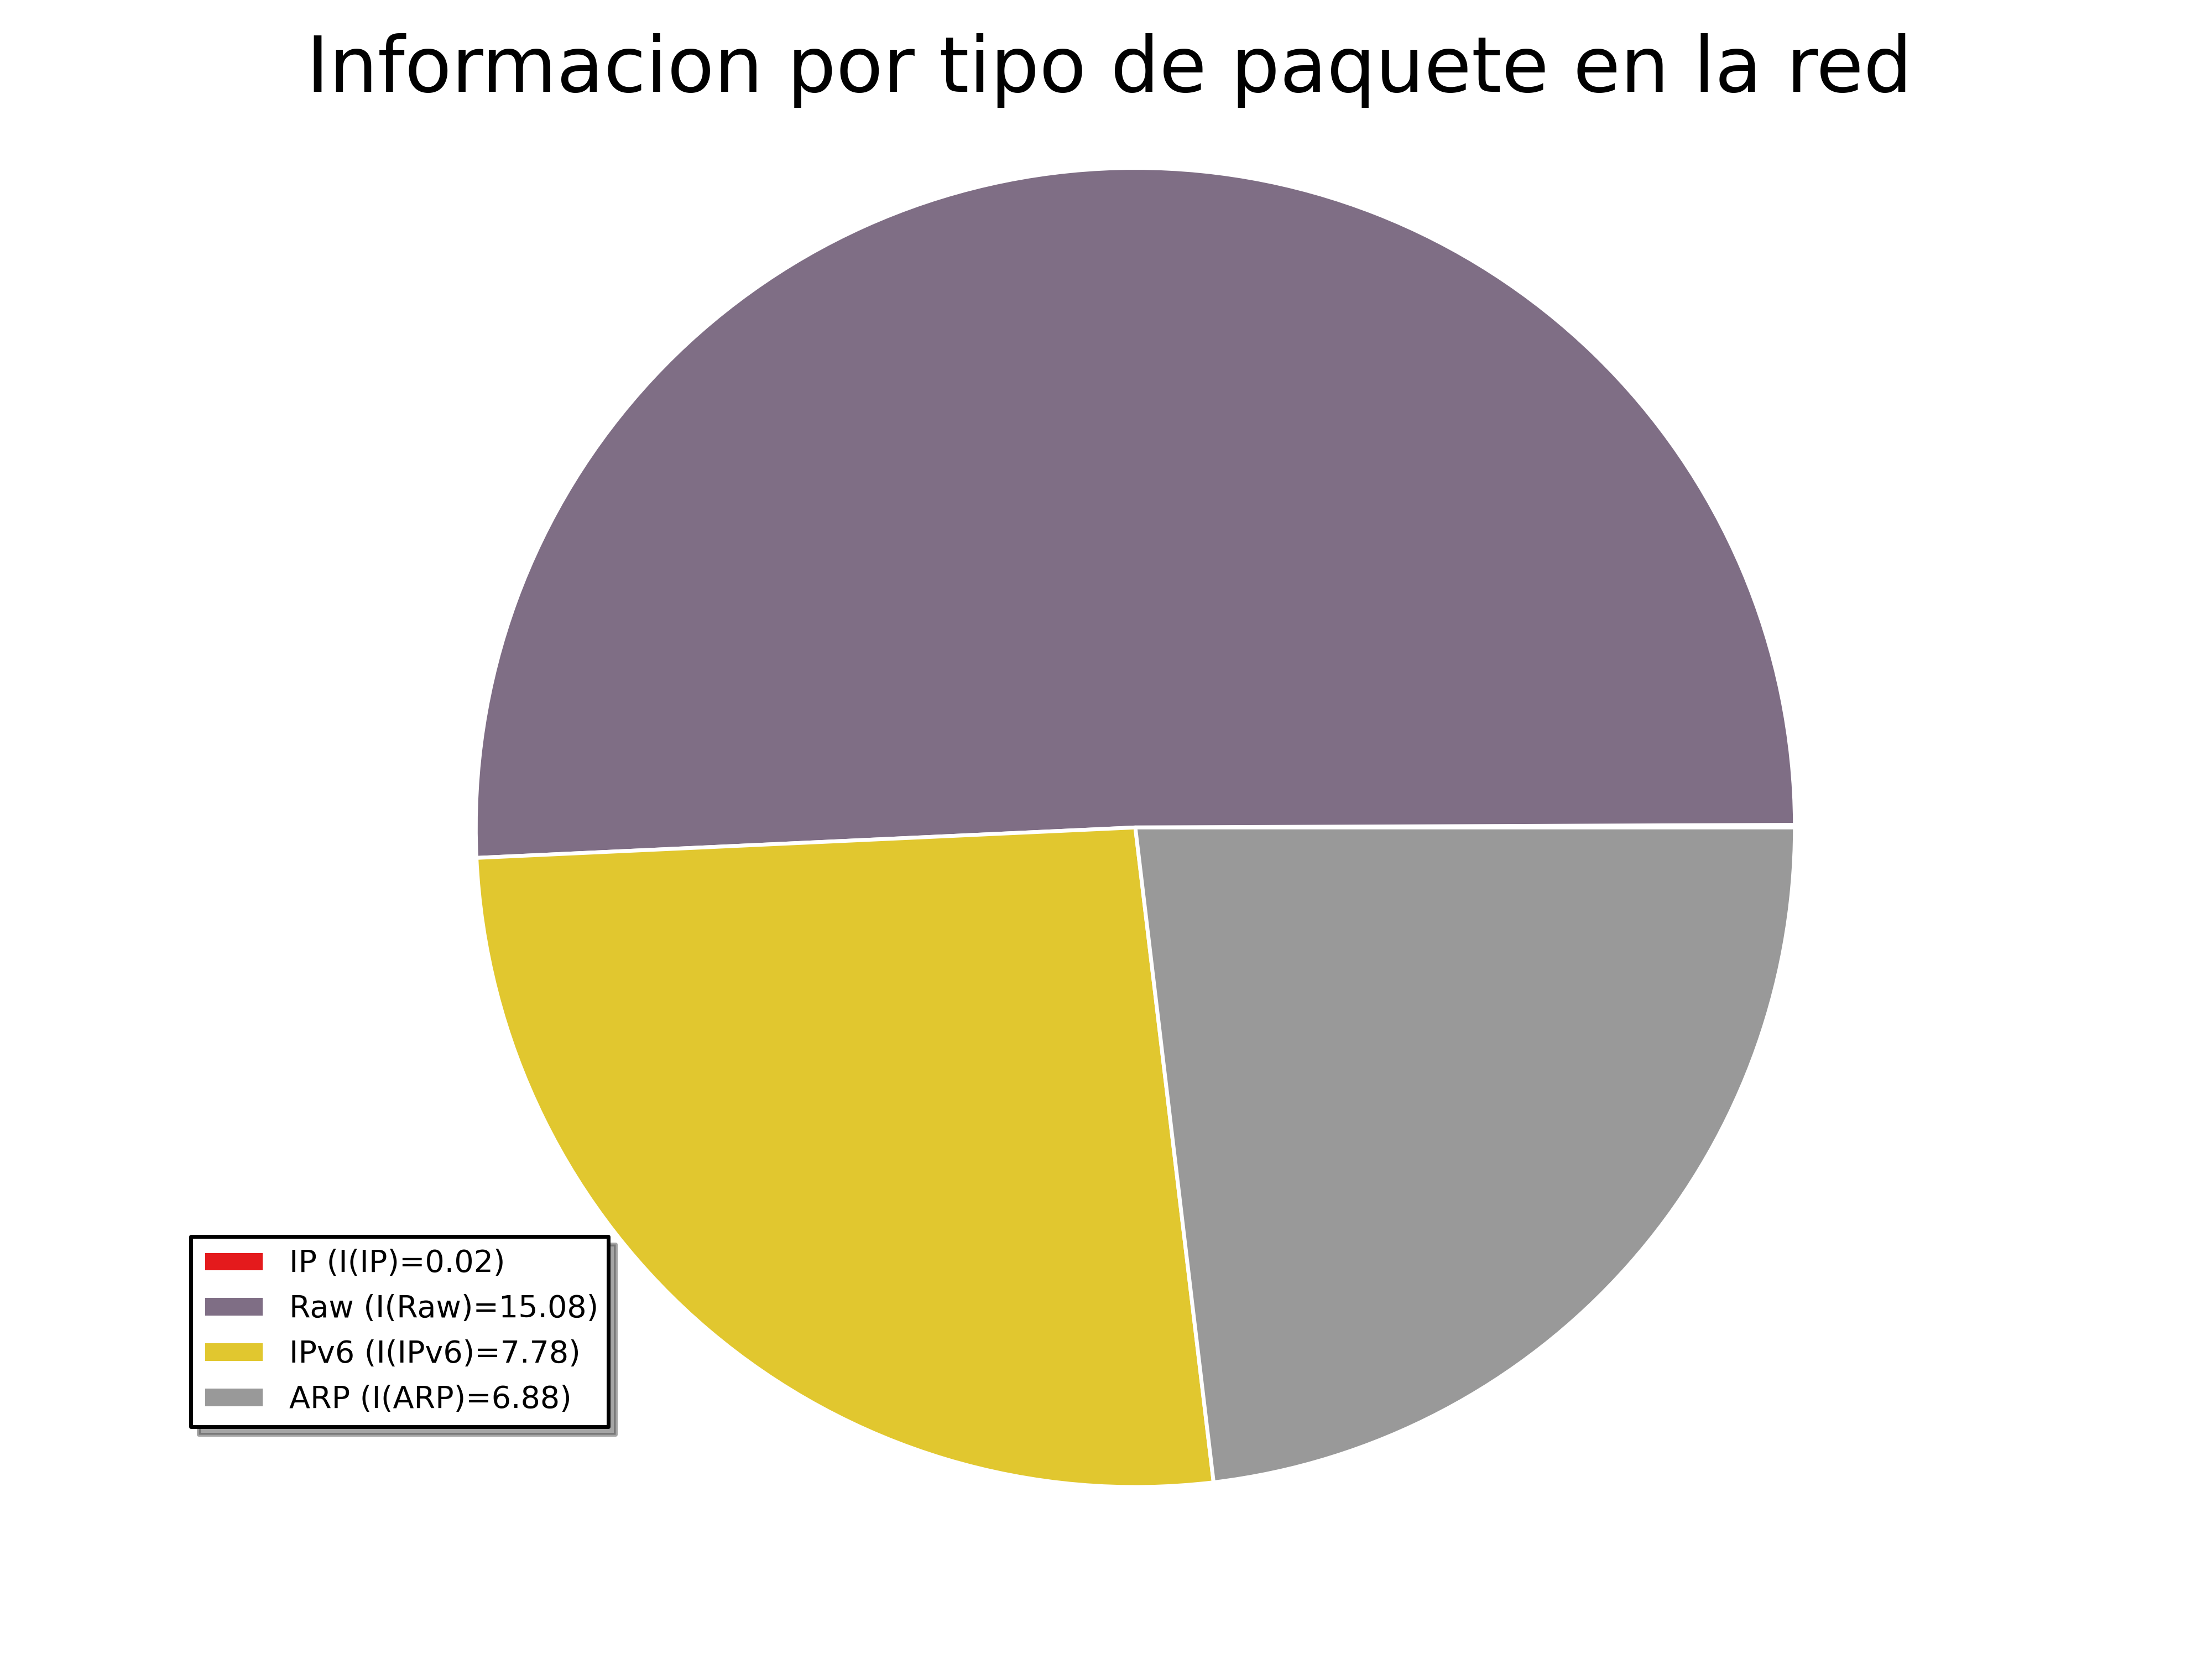
\includegraphics[width=\textwidth]{graficos/red_domestica_pie_type_information.png}
    \caption{Fuente $S$}
    \label{fig:red_domestica_pie_type_information}
  \end{minipage}
\end{figure}

En los gráficos Figura ~\ref{fig:red_domestica_pie_type}. y Figura ~\ref{fig:red_domestica_pie_type_information}. se puede observar que el protocolo que presenta mayor frecuencia es el IPv4 con un porcentaje muy superior al resto y que, por el contrario, aporta muy poca información. Por lo tanto, en este caso, el símbolo distinguido en la fuente $S$ sería el que representa al tipo de paquete IPv4.
\\
Podemos observar que, para este caso, la incidencia de los paquetes ARP en la red es baja en comparación al resto de los protocolos.
\\
\\
\FloatBarrier

Ahora veremos la relación entre la cantidad de paquetes y la información que proporciona cada nodo en la red para la fuente $S_1$. 

\begin{figure}[ht!]
  \centering
  \begin{minipage}[b]{0.48\textwidth}
    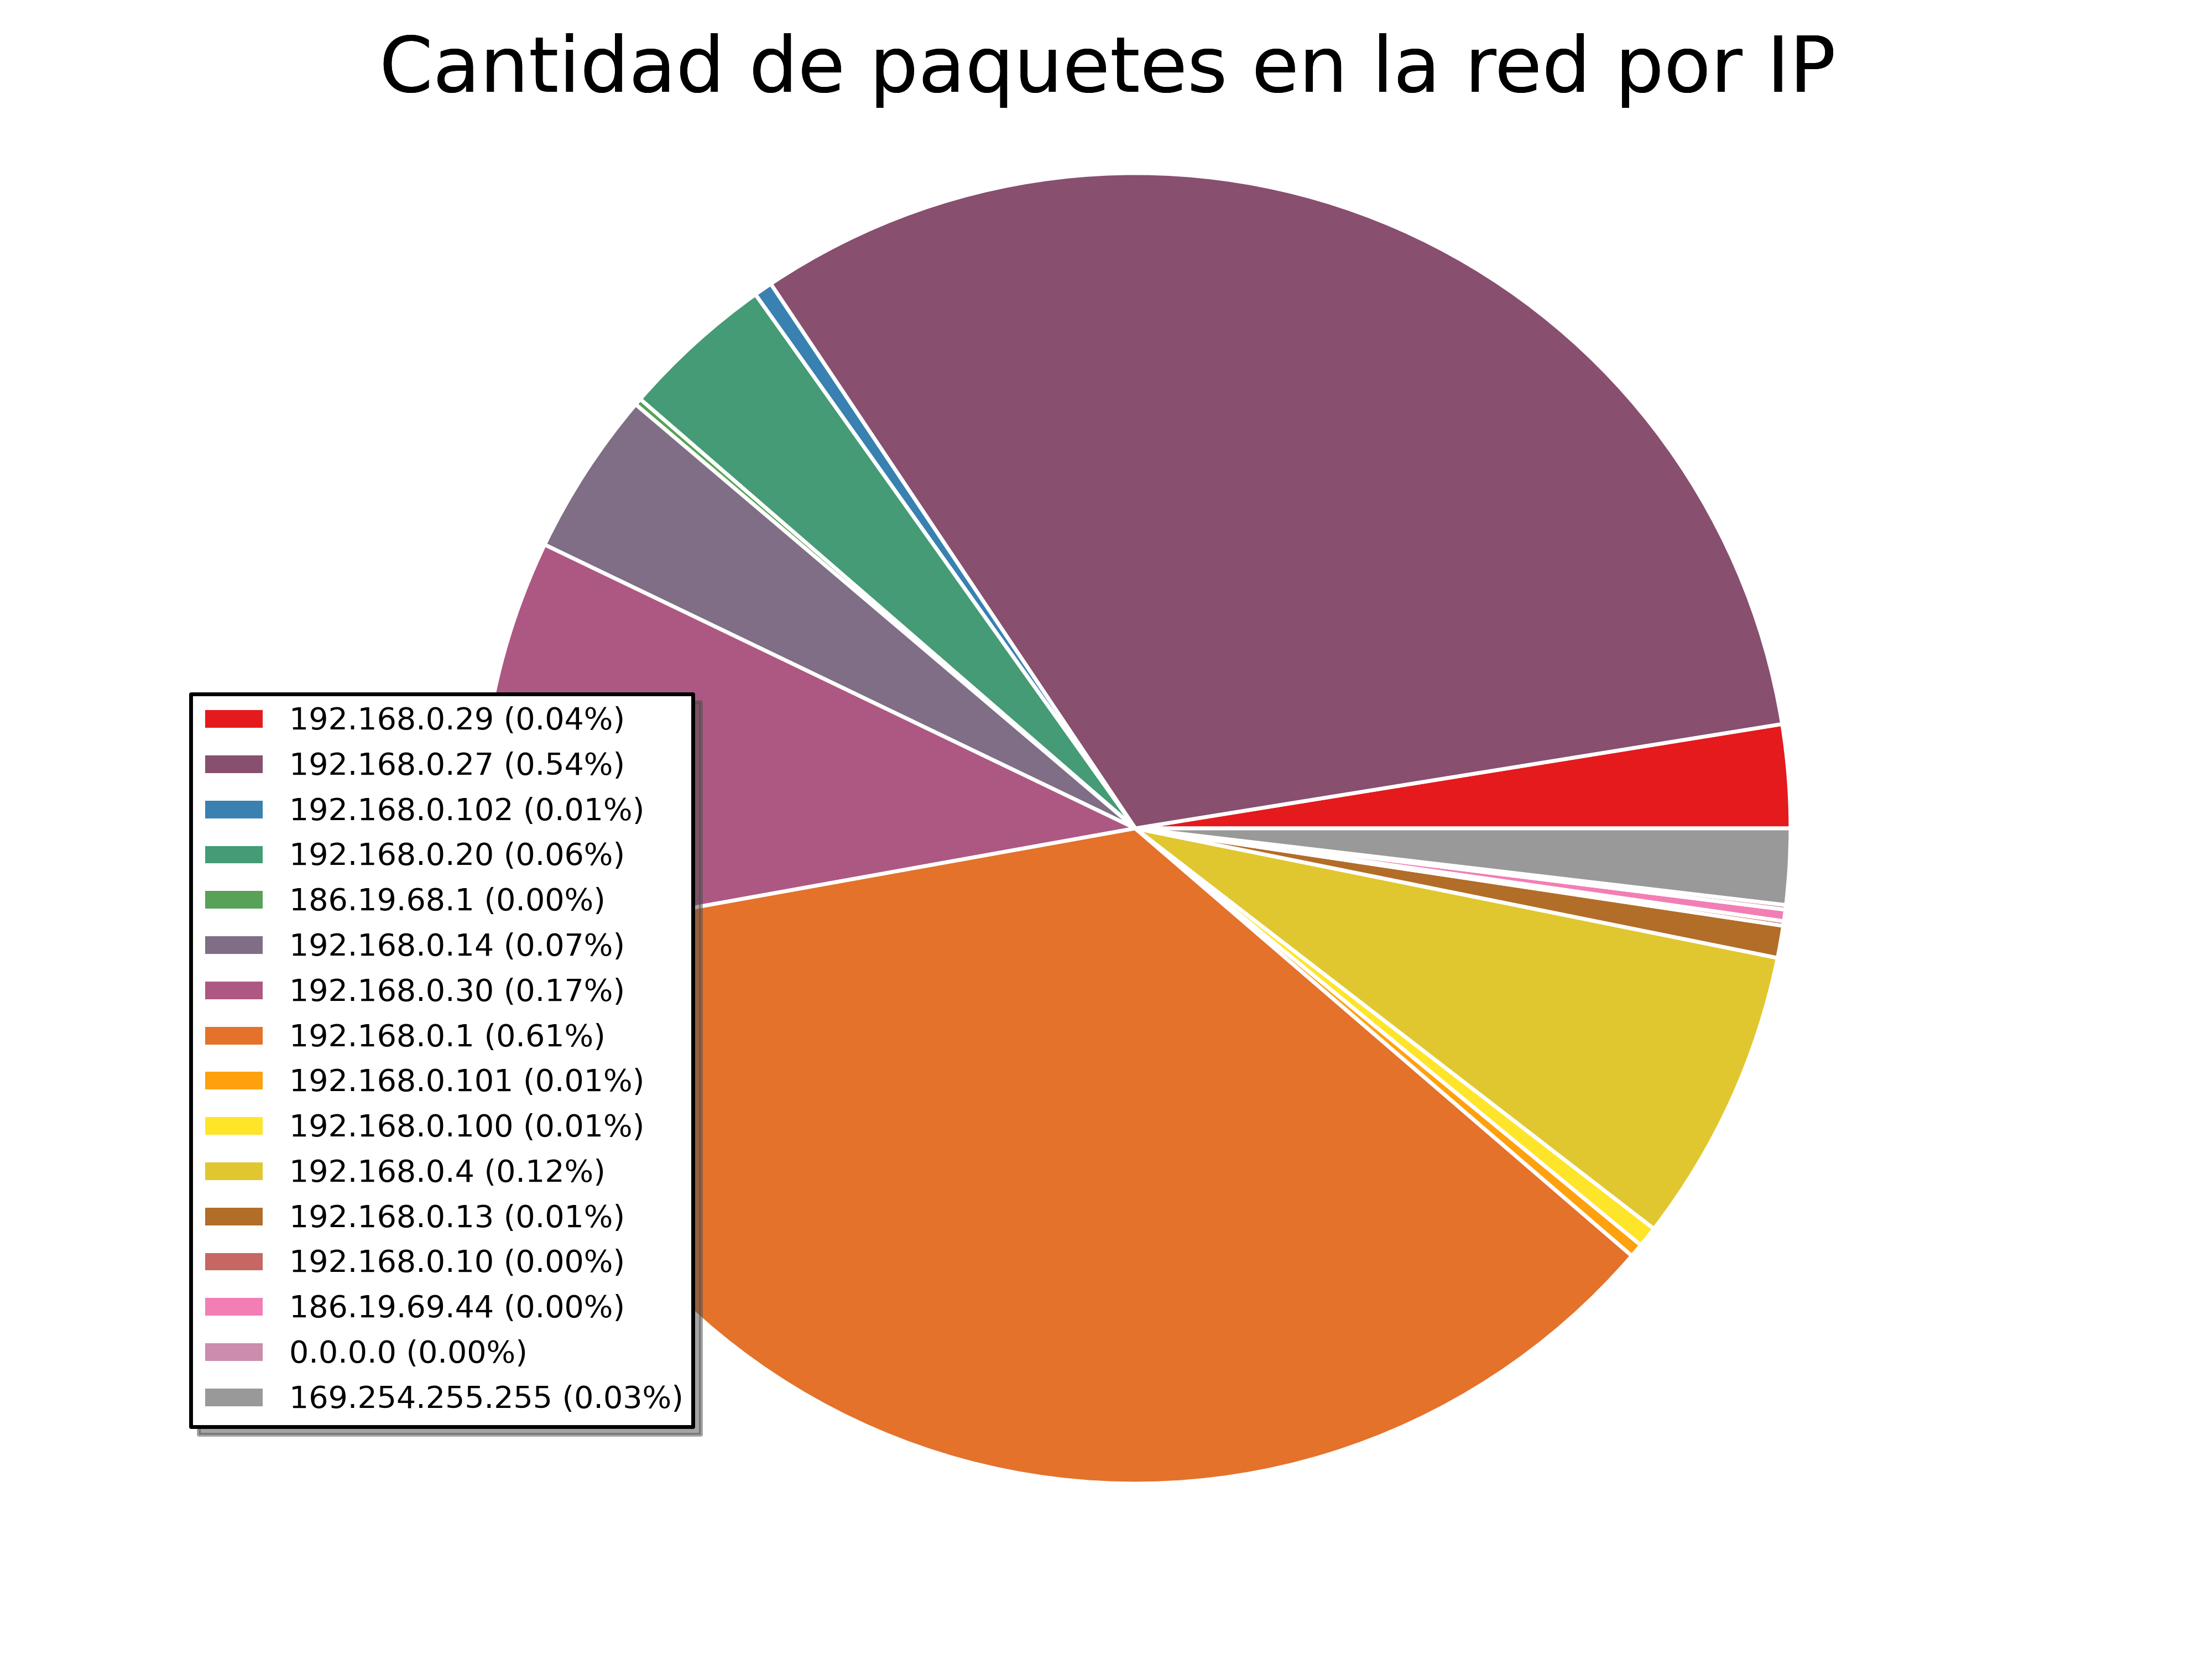
\includegraphics[width=\textwidth]{graficos/red_domestica_pie_arp.png}
    \caption{Fuente $S_1$}
    \label{fig:red_domestica_pie_arp}
  \end{minipage}
  \hfill
  \begin{minipage}[b]{0.48\textwidth}
    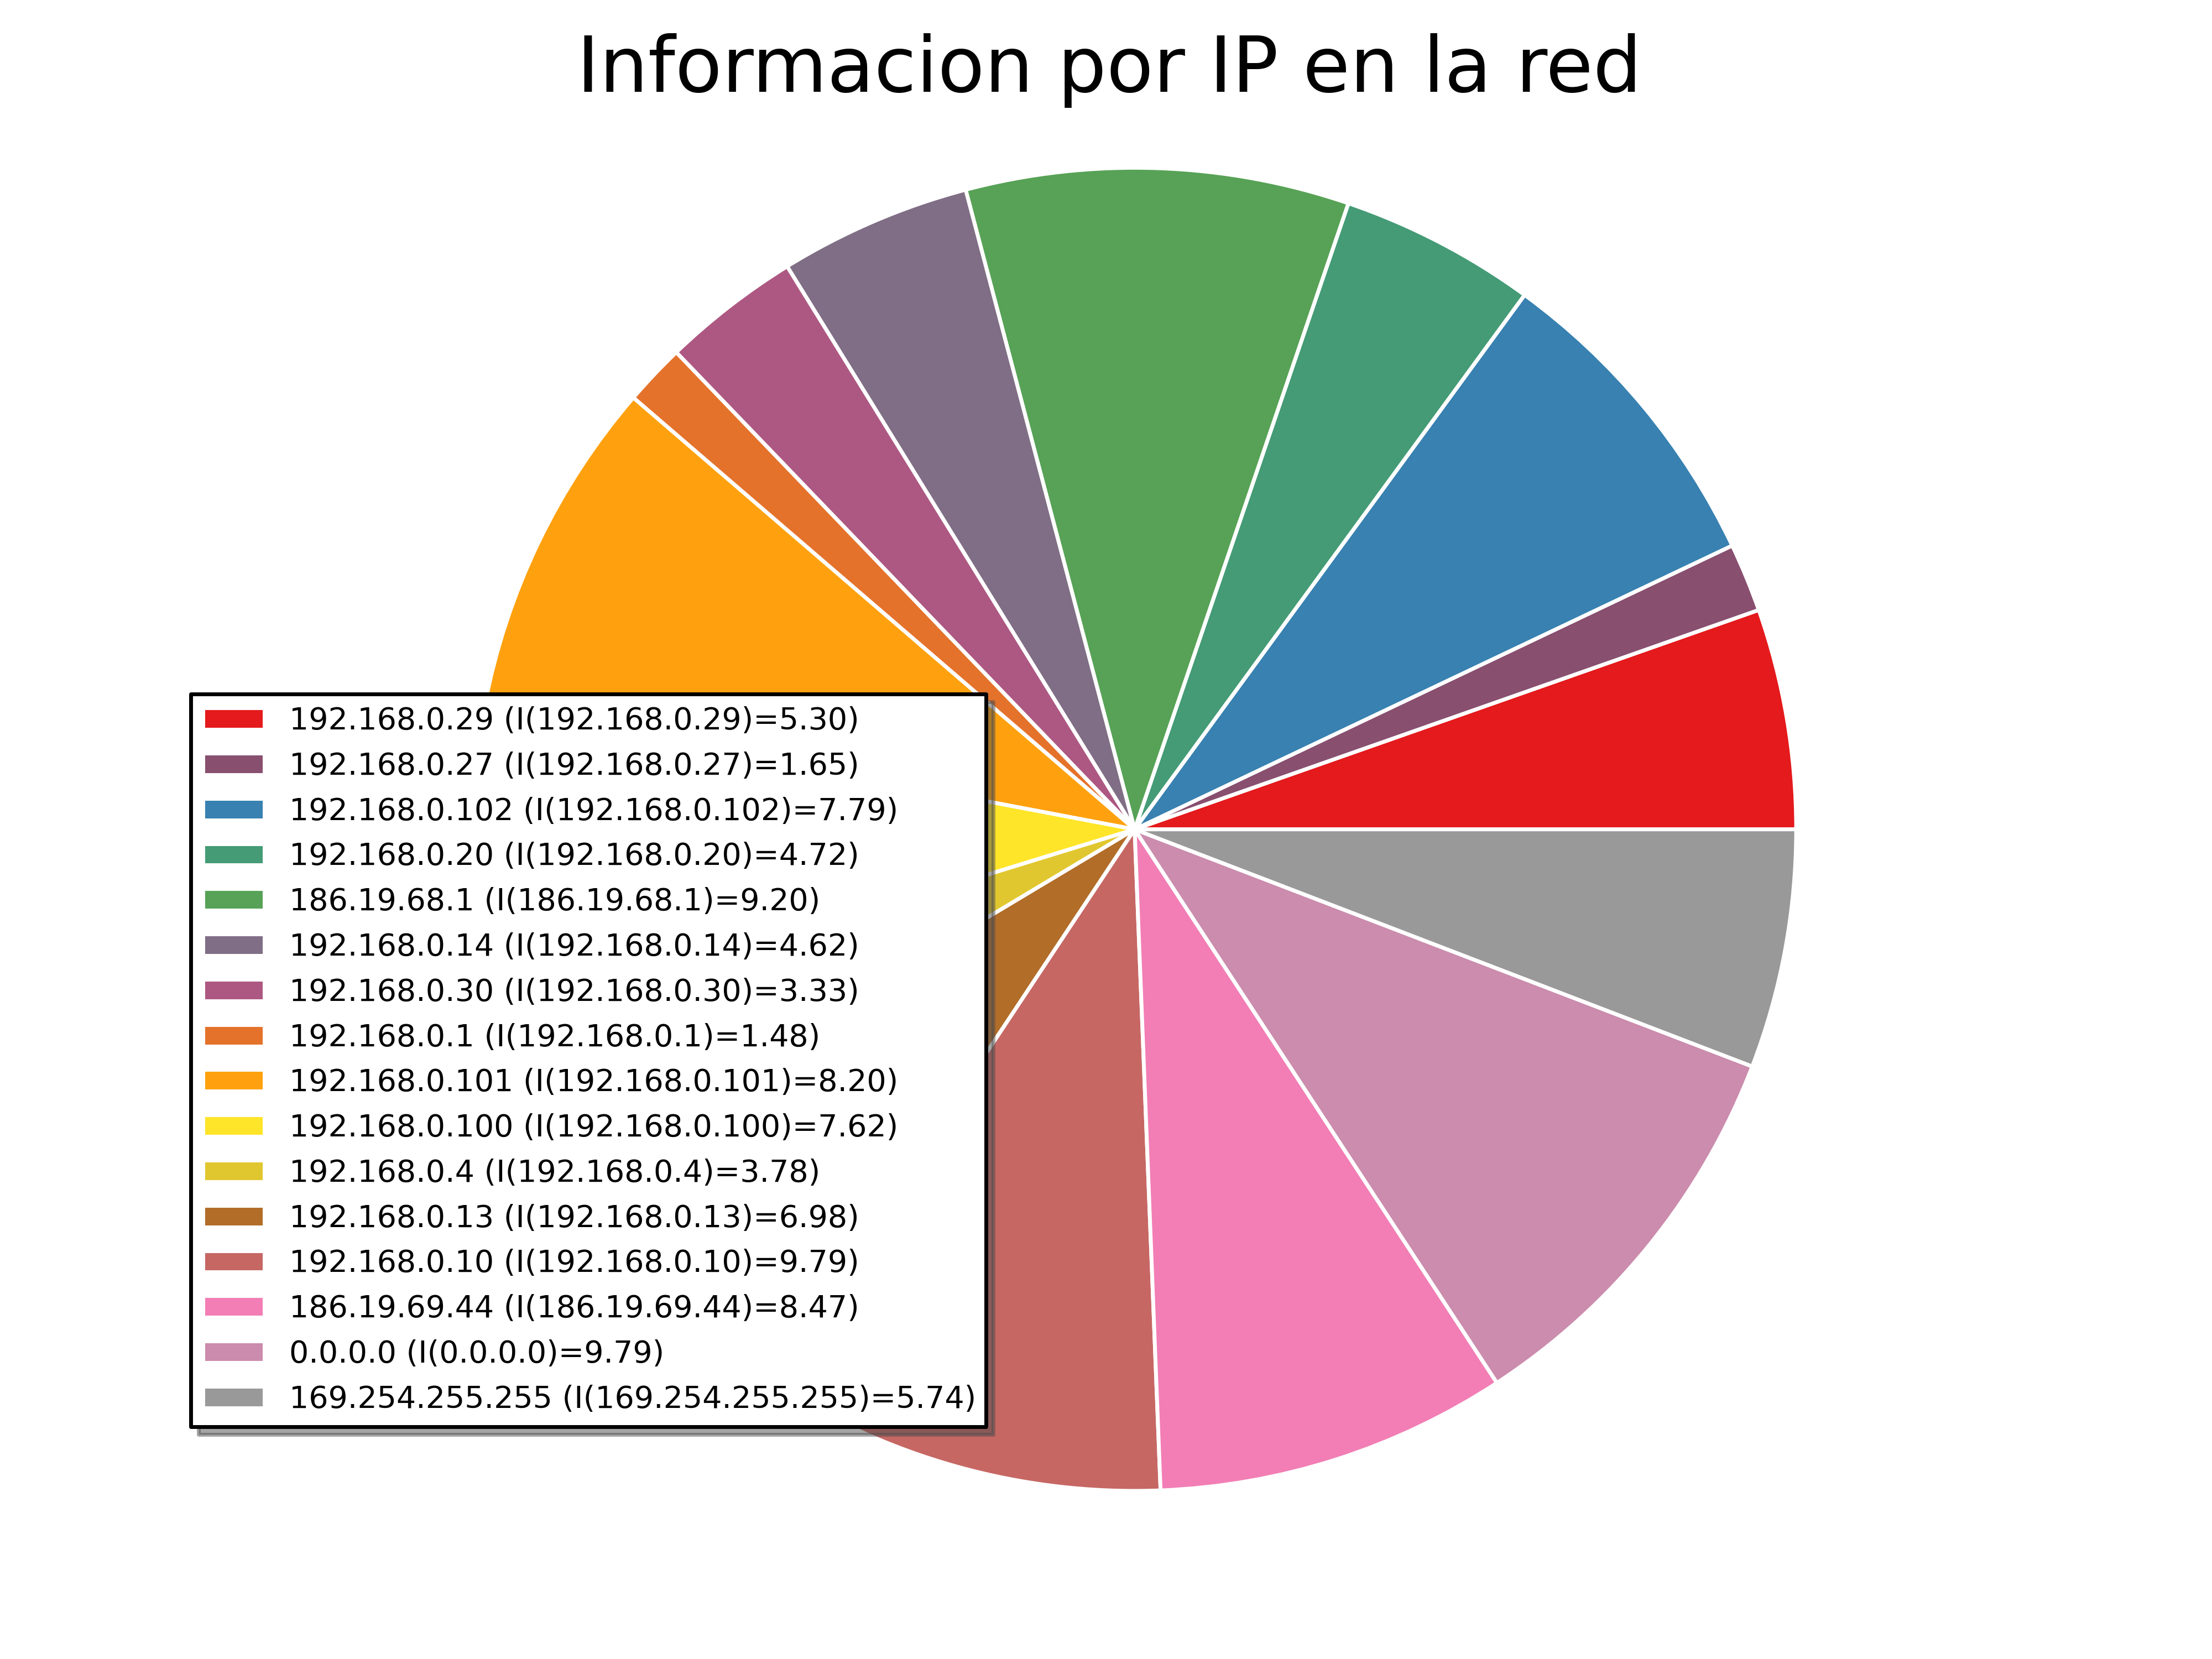
\includegraphics[width=\textwidth]{graficos/red_domestica_pie_arp_information.png}
    \caption{Fuente $S_1$}
    \label{fig:red_domestica_pie_arp_information}
  \end{minipage}
\end{figure}

En los datos de los gráficos Figura ~\ref{fig:red_domestica_pie_arp}. y Figura ~\ref{fig:red_domestica_pie_arp_information}. se toma como fuente a las direcciones IP de la red.
Se puede observar que los nodos distinguidos de la red para la fuente $S_1$ son los que poseen las direcciones IP 192.168.0.1 y 192.168.0.27, ya que son los que presentan mayor frecuencia y, por lo tanto, los que menos información aportan.

\FloatBarrier

\subsubsection{Nodos de la red}

A continuación, en la Figura ~\ref{fig:red_domestica_network}. se pueden observar los diferentes nodos de la red asociados a sus direcciones IP. Los ejes que conectan a un par de nodos representan que entre ellos hubo algún envío de paquetes ARP. El tamaño de cada nodo es proporcional a la cantidad de paquetes que el mismo envió y recibió.

\begin{figure}[ht!]
  \centering
   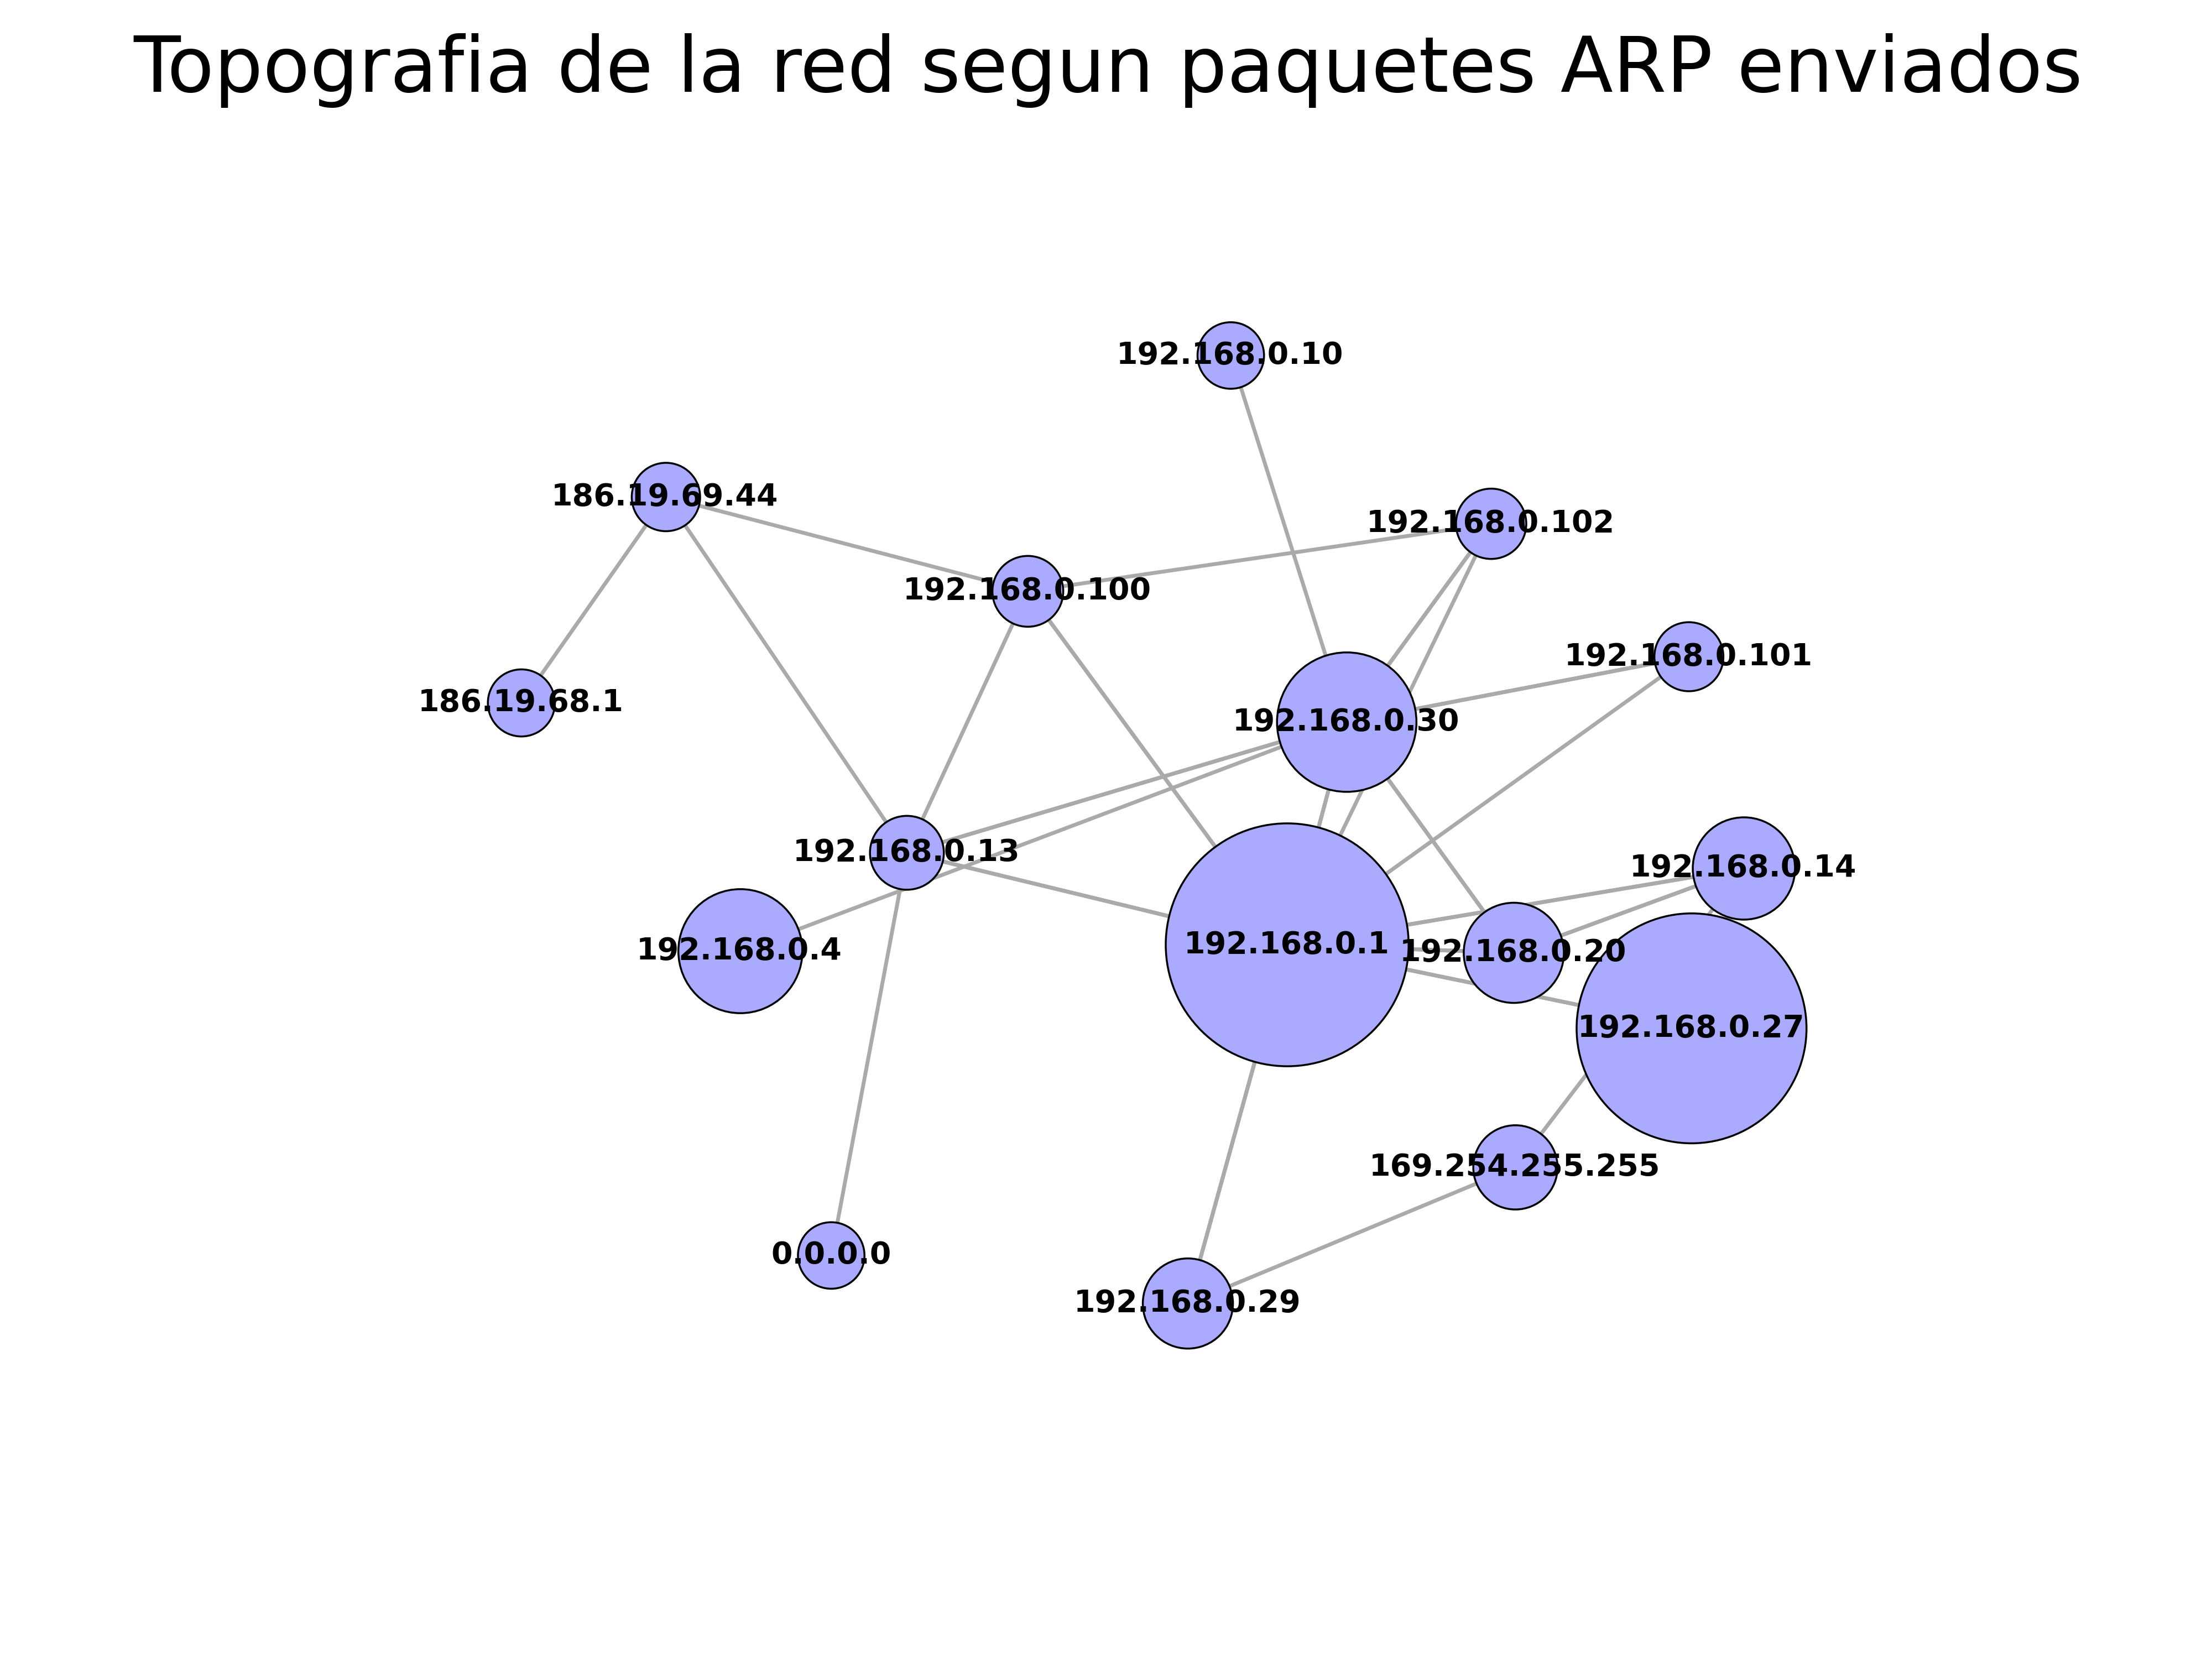
\includegraphics[width=0.7\textwidth]{graficos/red_domestica_network.png}
  \caption{}
  \label{fig:red_domestica_network}
\end{figure}

Al ser una red pequeña podemos confirmar claramente cuales son los nodos distinguidos: El que posee la dirección IP 192.168.0.1 que corresponde al modem y el host 192.168.0.27 correspondiente al SmartTV, que en el momento de la captura de los paquetes, el mismo se encontraba realizando actualizaciones.

\FloatBarrier

\subsubsection{Análisis de la de entropía}

A continuación analizaremos histogramas con cortes en los valores de entropía, tanto para las IP de la red como para los tipos de protocolo.

\begin{figure}[ht!]
  \centering
  \begin{minipage}[b]{0.48\textwidth}
    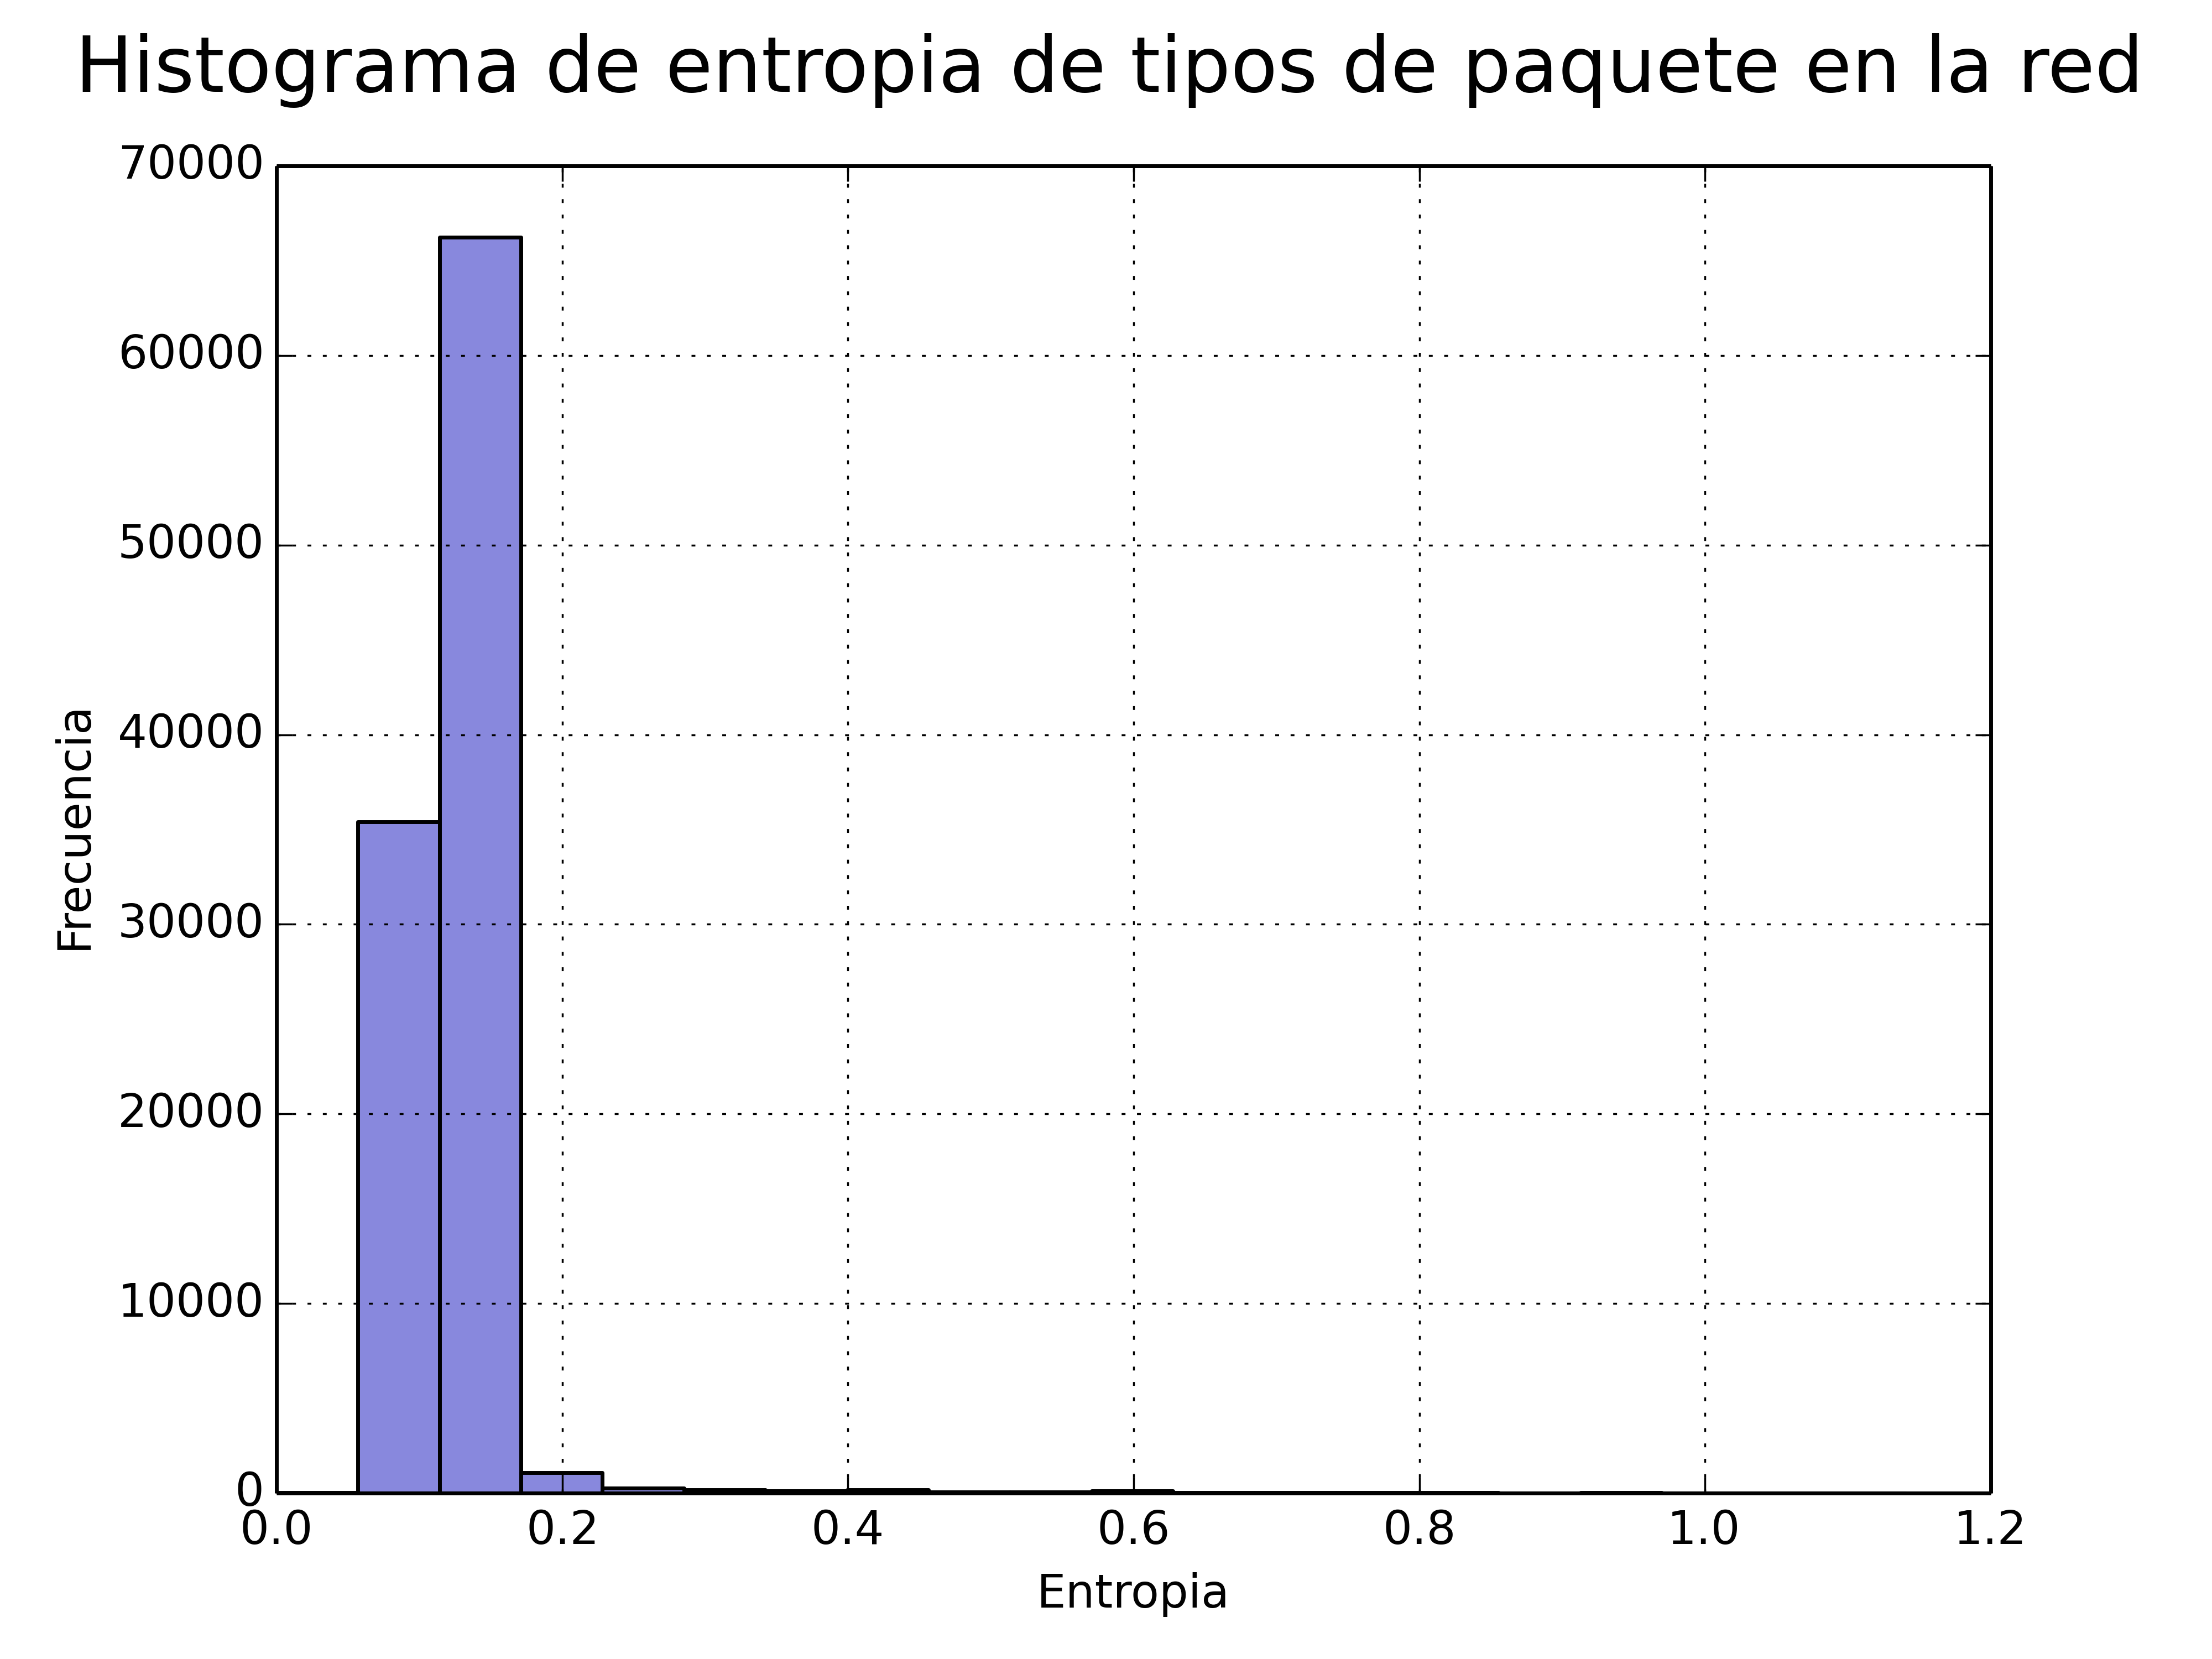
\includegraphics[width=\textwidth]{graficos/red_domestica_hist_type.png}
    \caption{Fuente $S$}
    \label{fig:red_domestica_hist_type}
  \end{minipage}
  \hfill
  \begin{minipage}[b]{0.48\textwidth}
    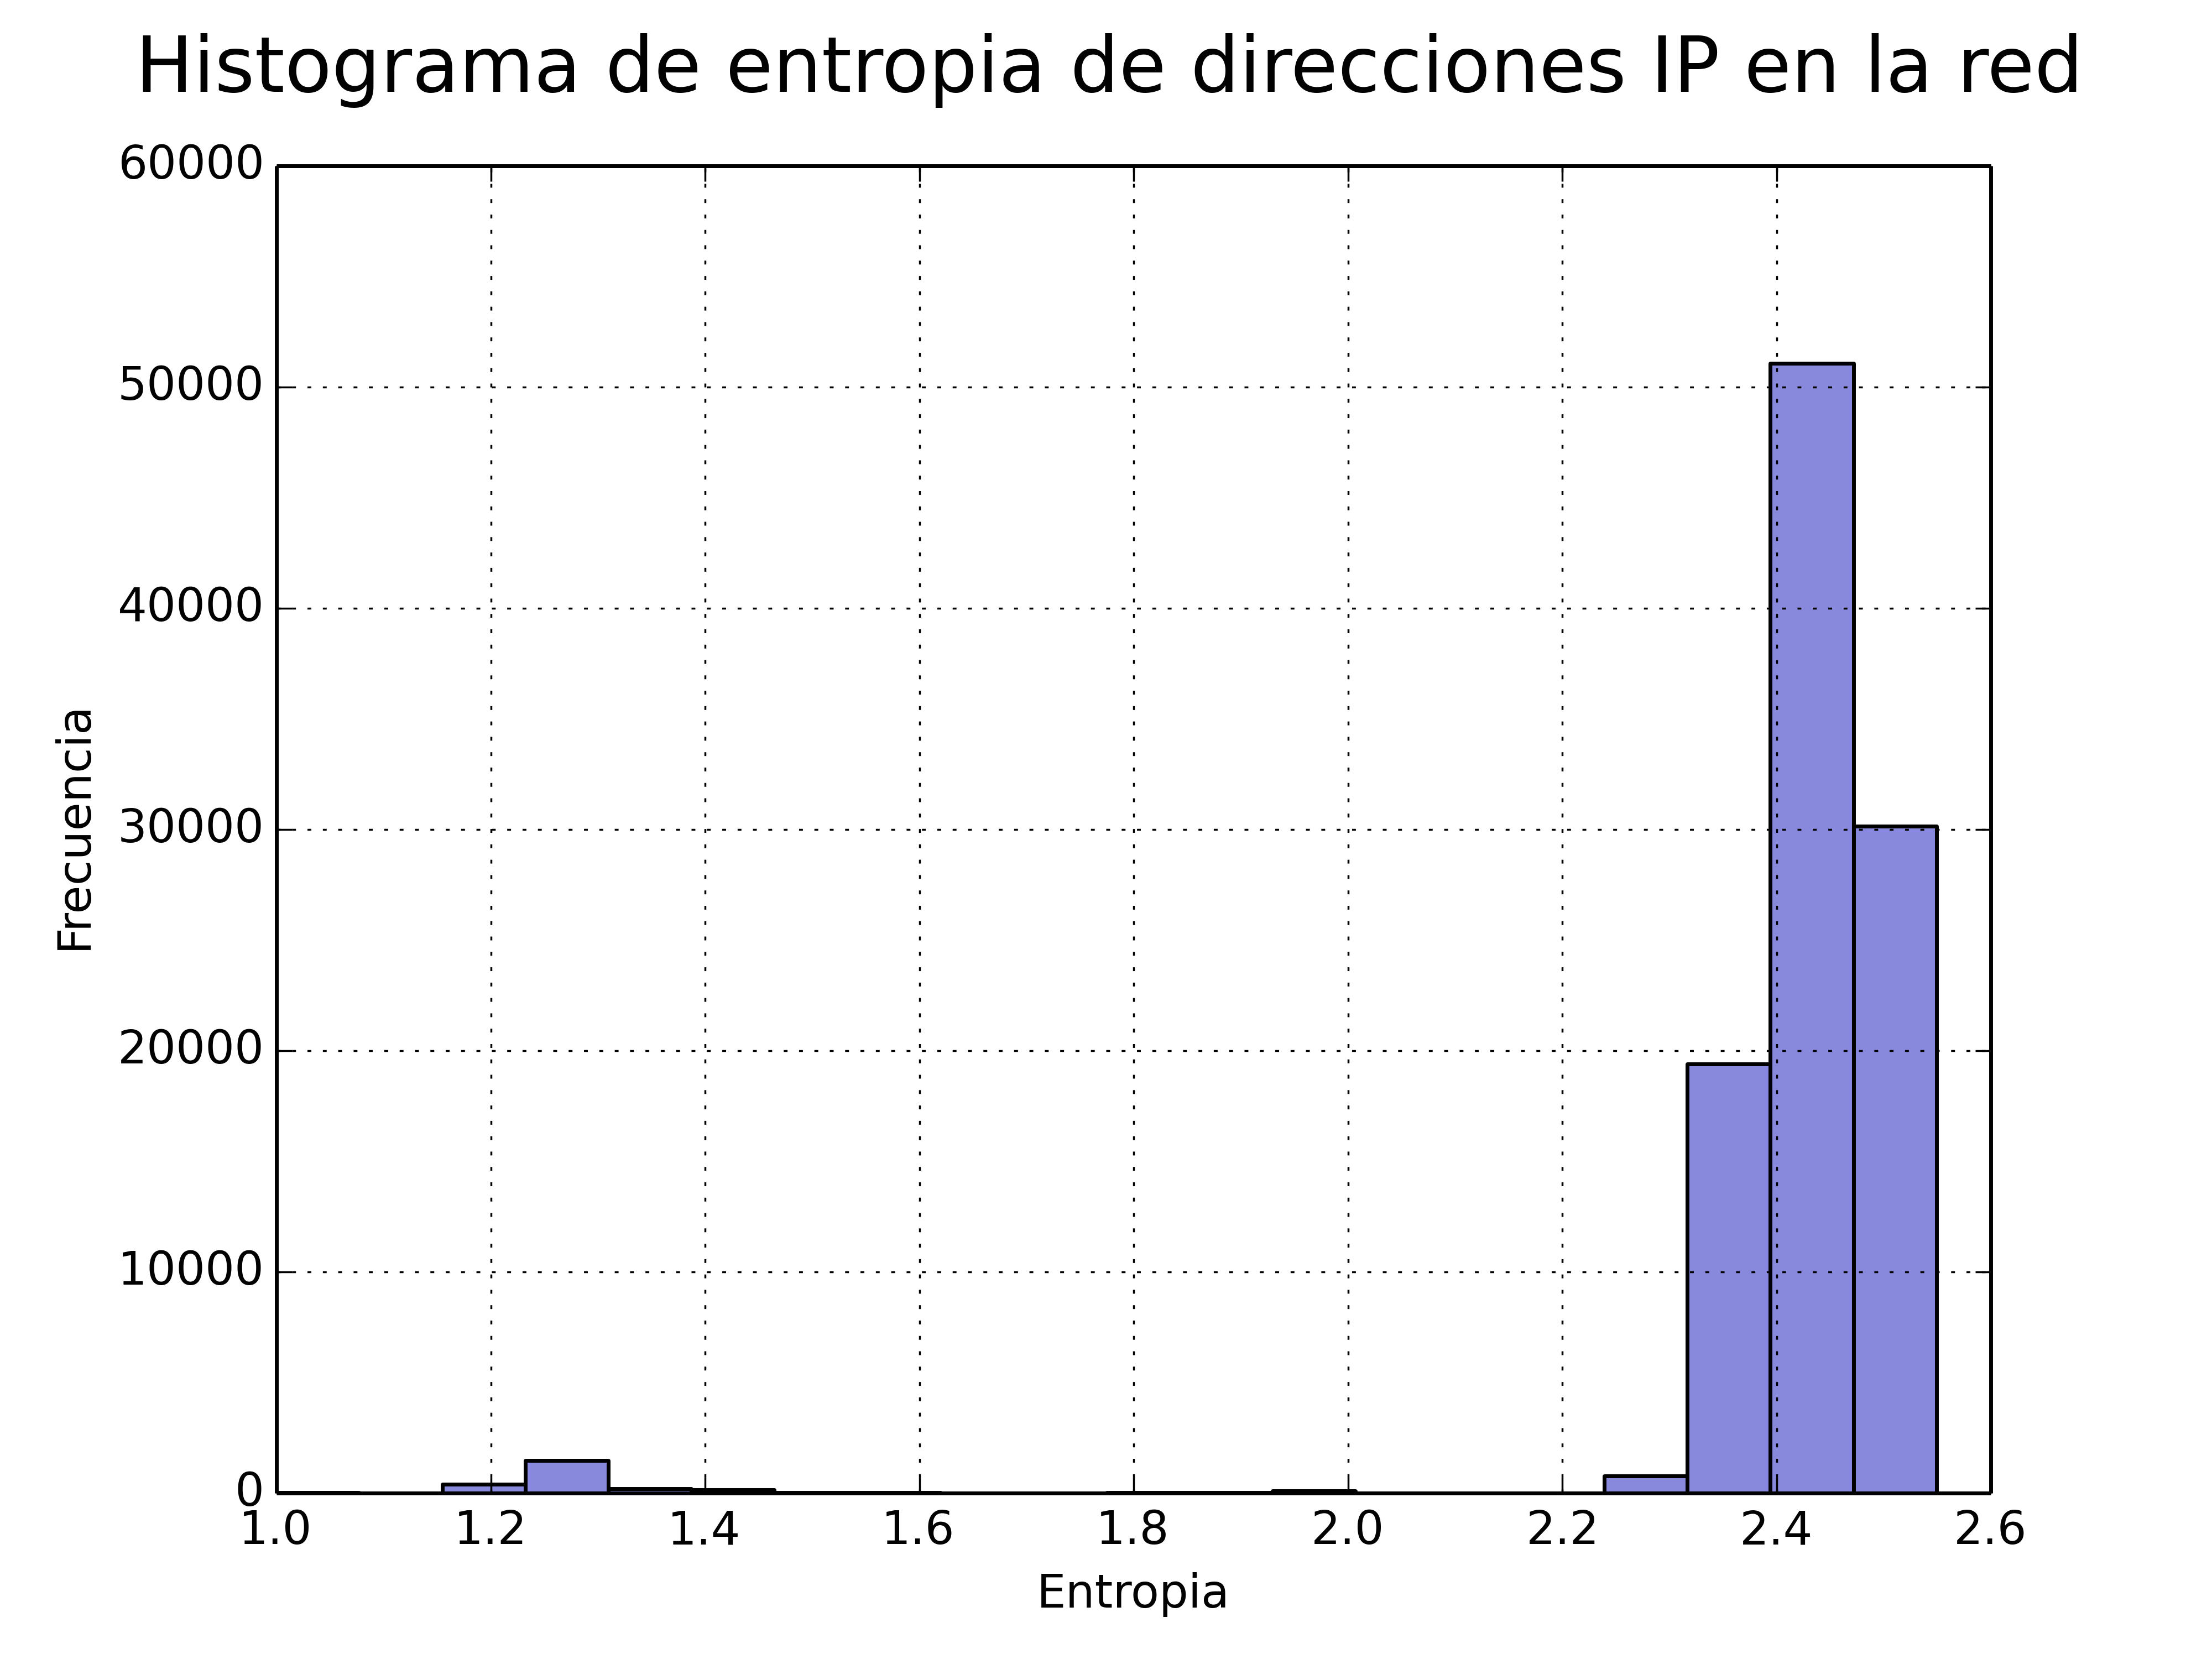
\includegraphics[width=\textwidth]{graficos/red_domestica_hist_arp.png}
    \caption{Fuente $S_1$}
    \label{fig:red_domestica_hist_arp}
  \end{minipage}
\end{figure}

Podemos observar que para el caso de la captura de paquetes de la fuente $S_1$ se presenta una entropía media mayor que en la fuente $S$. Esto se debe a la impredecibilidad de los símbolos en el caso de las direcciones IP en comparación con la de los tipos de protocolo, donde la mayoría de los protocolos de los paquetes fueron de tipo IPv4.